\documentclass[11pt,a4paper]{article}

\usepackage[T1]{fontenc}
\usepackage[utf8]{inputenc}
\usepackage{lmodern}
\usepackage[scaled=0.95]{inconsolata}
\usepackage{microtype}
% Typewriter text: print "--" as two hyphens (command-line options), not as a dash.
\DisableLigatures[-]{encoding = *, family = tt*}
\usepackage[margin=2.3cm]{geometry}
\usepackage{xcolor}
\usepackage{listings}
\usepackage{booktabs}
\usepackage{tabularx}
\usepackage{longtable}
\usepackage{multirow}
\usepackage{enumitem}
\usepackage{caption}
\usepackage[section]{placeins}   % floats stay within their section
\usepackage{amssymb}
\usepackage[most]{tcolorbox}
\usepackage{fancyhdr}
\usepackage{tikz}
\usetikzlibrary{positioning,arrows.meta,fit}
\usepackage[hidelinks]{hyperref}

% ---------------------------------------------------------------------------
% Text elements are black and white (same style as ../install-guide). Color
% is used only for the syntax highlighting of code, on a transparent
% background.
% ---------------------------------------------------------------------------
\definecolor{kw}{RGB}{0,70,160}       % keywords
\definecolor{cmt}{RGB}{90,110,90}     % comments
\definecolor{str}{RGB}{160,60,30}     % strings
\definecolor{lnum}{gray}{0.55}        % line numbers

\newtcolorbox{note}{enhanced,breakable,sharp corners,colback=white,colframe=black,
  boxrule=0pt,leftrule=0.8pt,left=8pt,right=0pt,top=2pt,bottom=2pt,
  before upper={\textbf{Note.}\ }}
\newtcolorbox{finding}[1]{enhanced,breakable,sharp corners,colback=white,colframe=black,
  boxrule=0pt,leftrule=0.8pt,left=8pt,right=0pt,top=2pt,bottom=2pt,
  before upper={\textbf{Finding #1.}\ }}

\newcommand{\yes}{\checkmark}
\newcommand{\no}{$\times$}
\newcommand{\ice}{ICE}

% ---------------------------------------------------------------------------
% Listings: transparent background, thin black rules above and below
% ---------------------------------------------------------------------------
\lstset{
  basicstyle=\ttfamily\small,
  frame=lines, framerule=0.4pt, rulecolor=\color{black},
  breaklines=true, breakatwhitespace=false,
  postbreak=\mbox{$\hookrightarrow$\space},
  columns=fullflexible, keepspaces=true,
  showstringspaces=false,
  xleftmargin=0pt, xrightmargin=0pt,
  aboveskip=8pt, belowskip=8pt,
  captionpos=b,
  upquote=true,
}
\lstdefinestyle{shell}{
  language=bash,
  keywordstyle=\color{kw},
  commentstyle=\color{cmt}\itshape,
  stringstyle=\color{str},
  morekeywords={opam,eval,jasminc,jasmin2ec,jasmin-ct,easycrypt,gcc,dune,python3,make},
}
\lstdefinestyle{output}{
  language={}, basicstyle=\ttfamily\scriptsize,
}
\lstdefinelanguage{Jasmin}{
  morekeywords={fn,export,inline,return,reg,stack,int,bool,u8,u16,u32,u64,
    u128,u256,for,to,downto,while,if,else,param,global,require,from,ptr},
  sensitive=true,
  morecomment=[l]{//},
  morecomment=[s]{/*}{*/},
  morecomment=[s]{\#[}{]},
  morestring=[b]",
}
\lstdefinestyle{jasmin}{
  language=Jasmin, keywordstyle=\color{kw}\bfseries,
  commentstyle=\color{cmt}\itshape, stringstyle=\color{str},
  numbers=left, numberstyle=\tiny\color{lnum}, numbersep=6pt,
  basicstyle=\ttfamily\footnotesize,
}
\lstdefinelanguage{EasyCrypt}{
  morekeywords={require,import,from,lemma,proof,qed,module,proc,var,return,
    hoare,equiv,phoare,op,type,axiom,theory,end,clone,with,as,if,then,else,
    forall,exists,fun,by,smt,ring,rnd,skip,wp,rewrite,have,split,first,move,
    admit,res,true,false,while,sim,inline,auto,case,apply,done},
  sensitive=true,
  morecomment=[s]{(*}{*)},
  morestring=[b]",
}
\lstdefinestyle{easycrypt}{
  language=EasyCrypt, keywordstyle=\color{kw}\bfseries,
  commentstyle=\color{cmt}\itshape, stringstyle=\color{str},
  numbers=left, numberstyle=\tiny\color{lnum}, numbersep=6pt,
  basicstyle=\ttfamily\footnotesize,
}
\lstdefinestyle{asm}{
  language={}, morekeywords={adds,adcs,adc,ldr,str,stp,ldp,movz,ret,blr,cmp,cset,lsl,orr,add,fmov,mov,sub},
  keywordstyle=\color{kw}, morecomment=[l]{//}, commentstyle=\color{cmt}\itshape,
  basicstyle=\ttfamily\footnotesize,
}
\lstdefinestyle{c}{
  language=C, keywordstyle=\color{kw}\bfseries,
  commentstyle=\color{cmt}\itshape, stringstyle=\color{str},
  numbers=left, numberstyle=\tiny\color{lnum}, numbersep=6pt,
  basicstyle=\ttfamily\footnotesize,
}
\lstdefinestyle{ocaml}{
  language=[Objective]Caml, keywordstyle=\color{kw}\bfseries,
  commentstyle=\color{cmt}\itshape, stringstyle=\color{str},
  numbers=left, numberstyle=\tiny\color{lnum}, numbersep=6pt,
  basicstyle=\ttfamily\footnotesize,
}
\lstdefinestyle{python}{
  language=Python, keywordstyle=\color{kw}\bfseries,
  commentstyle=\color{cmt}\itshape, stringstyle=\color{str},
  numbers=left, numberstyle=\tiny\color{lnum}, numbersep=6pt,
  basicstyle=\ttfamily\footnotesize,
}

\newcommand{\cmd}[1]{\lstinline[style=shell,frame=none]{#1}}
\newcommand{\file}[1]{\texttt{#1}}

\pagestyle{fancy}
\fancyhf{}
\lhead{\small Test campaign of the Jasmin ARMv8-A back end on the Raspberry Pi 5}
\rhead{\small\thepage}

\title{\textbf{Testing the Jasmin ARMv8-A Back End\\on the Raspberry Pi 5}\\[4pt]
  \large Differential, ABI, cryptographic, constant-time and EasyCrypt validation\\
  of Jasmin 2026.09.0 and EasyCrypt r2026.07}
\author{}
\date{October 21, 2026}

\begin{document}
\maketitle
\thispagestyle{empty}

\begin{abstract}
\noindent
Jasmin 2026.09.0 is the first release whose verified compiler generates
code for ARMv8-A (AArch64), the 64-bit Arm architecture. The upstream test
suite of Jasmin verifies only that the ARMv8-A test programs
\emph{compile}; it does not execute the generated code. This report
describes a test campaign, conducted entirely on a Raspberry Pi~5
(Cortex-A76), that executes the generated code natively and compares its
results with several independent references: the reference interpreter of
Jasmin, hand-written C models, built-in functions of GCC, the test vectors
of RFC~8439, and the OpenSSL library. The campaign also examines the
AAPCS64 calling convention, the erasure of secrets from the stack, and
constant-time security (with the checker \texttt{jasmin-ct}, with timing
measurements, and with EasyCrypt proofs on the extracted leakage model), and
it proves in EasyCrypt the functional correctness of the carry handling.
All \textbf{161 checks pass} in 7 minutes. More than 10 million executions
of generated code reveal \textbf{no miscompilation}, that is, no case in
which the compiled code computes a result different from the one that the
language semantics prescribes. The report also documents 17 limitations of
the back end. Three of them are internal compiler errors (for the
operations \texttt{mulu} and the 32-bit \texttt{swap}). Speculative load
hardening, a protection against Spectre attacks, is accepted by the checker
but rejected by the compiler. The instructions \texttt{UMULL} and
\texttt{UMADDL} are defined in the EasyCrypt model but not available in the
compiler, which makes Poly1305 2.5 times slower than C. Each limitation is
accompanied by a workaround that has been tested.
\end{abstract}

\tableofcontents
\newpage

%===========================================================================
\section{Introduction}
%===========================================================================

The companion document \file{../install-guide} describes the installation of
Jasmin and EasyCrypt on a Raspberry Pi~5 and a set of smoke tests. The
present document addresses two further questions: \emph{can the new ARMv8-A
back end be trusted, and which programs does it currently support?} The
reader is assumed to have read the installation guide or to be familiar with
its content; terms that it does not introduce are explained below and in the
glossary (Appendix~\ref{app:glossary}).

\subsection{Why test a verified compiler?}

The correctness of the Jasmin compiler is proved in Coq: for every program
that the compiler accepts, the generated code has the same behavior as the
source program.
This proof covers the compiler passes, but not every component on which a
user relies. It does not cover the OCaml components that are not extracted
from Coq (the parser and some auxiliary algorithms written in OCaml), the
printing of the
assembly text, the assumptions about the semantics of the processor
instructions, the platform ABI (the conventions by which separately compiled
functions interoperate), or the assembler and linker. Moreover, the proof
does not specify which source programs the back end accepts. Testing on real
hardware complements the proof in all these respects.

\subsection{Terms used in this report}

\begin{description}[leftmargin=0pt,itemsep=2pt]
  \item[Back end] The part of the compiler that generates code for one
        processor architecture, here ARMv8-A.
  \item[Miscompilation] A case in which the compiled code computes a result
        that differs from the result that the language semantics
        prescribes.
  \item[Oracle] An independent source of expected results against which a
        test compares the results of the code under test.
  \item[Differential testing] Testing that executes two implementations of
        the same function on the same inputs and compares their results.
  \item[AAPCS64] The procedure call standard of AArch64, which specifies how
        functions receive arguments and return results, and which registers
        they must preserve.
  \item[Constant time, leakage] A program is constant-time if secret data
        influence neither its control flow nor its memory addresses. The
        \emph{leakage} of an execution is the sequence of its branch
        decisions and memory addresses, which determine its timing and which
        an attacker who measures time may therefore learn.
  \item[Spectre v1, SLH] Spectre v1 is an attack that exploits the
        speculative execution of conditional branches. Speculative load
        hardening (SLH) is a programming technique that protects against
        it.
  \item[ICE] Internal compiler error: the compiler fails with an internal
        error instead of producing code or a diagnostic for the user.
\end{description}

\subsection{Objectives and structure}

The campaign consists of eight stages, each of which has its own directory
and its own section in this report. Each section states the purpose of the
stage, describes the method, and presents the results. Problems of the back
end are highlighted as \emph{findings}.

\begin{enumerate}[leftmargin=*,itemsep=1pt]
  \item Compile the upstream ARMv8-A tests and the architecture-independent
        tests for the ARMv8-A target (Stage~1).
  \item Execute the compiled code and compare its results with the language
        semantics by \emph{differential testing} (Stage~2).
  \item Verify the AAPCS64 calling convention and the erasure of secrets
        from the stack on the target machine (Stage~3).
  \item Implement two cryptographic primitives (ChaCha20, Poly1305) and
        validate them against the standard and against OpenSSL (Stage~4).
  \item Validate the constant-time guarantees statically, empirically and
        formally (Stages~5--6).
  \item Measure performance (Stage~7) and catalog the limitations of the
        back end (Stage~8).
\end{enumerate}

\subsection{Summary of results}

Table~\ref{tab:summary} lists the checks of each stage. A check is a single
pass/fail decision of the test script; the complete output of a run is
reproduced in Appendix~\ref{app:output}.

\begin{table}[h]
\centering\small
\begin{tabularx}{\textwidth}{@{}clXr@{}}
\toprule
\textbf{Stage} & \textbf{Topic} & \textbf{Content} & \textbf{Checks} \\
\midrule
1 & Upstream tests & 72 programs compiled and assembled, 27 test cases of the constant-time checker, 17 translations to EasyCrypt type-checked & 47 \\
2 & Differential testing & 35 functions $\times$ 2000--5000 inputs (interpreter vs native code), $2\times10^6$ tests against C models & 37 \\
3 & ABI & callee-saved registers, 32-bit arguments with undefined upper halves, erasure of secrets from the stack & 17 \\
4 & Cryptography & ChaCha20 and Poly1305: RFC 8439 test vectors, 262\,608 comparisons with OpenSSL & 4 \\
5 & Constant time & \texttt{jasmin-ct} (modes CT, DOIT, SCT), 200\,000 functional tests, 4 timing tests & 24 \\
6 & EasyCrypt & 10 extracted models, 2 correctness proofs and 5 constant-time proofs, 3 negative proofs & 15 \\
7 & Performance & ChaCha20 and Poly1305 compared with C and OpenSSL & info \\
8 & Limitations & 17 expected compilation failures & 17 \\
\midrule
  & \textbf{Total} & & \textbf{161 / 161} \\
\bottomrule
\end{tabularx}
\caption{Overview of the test campaign.}
\label{tab:summary}
\end{table}

\paragraph{Principal findings.}
\begin{itemize}[leftmargin=*,itemsep=1pt]
  \item \textbf{No miscompilation}: more than $10^7$ executions of
        Jasmin-generated AArch64 code agree with the reference semantics
        and with independent implementations.
  \item The generated code conforms to AAPCS64: it preserves the
        callee-saved registers and the stack pointer, and it ignores the
        undefined upper halves of 32-bit arguments. The erasure option of
        the compiler (stack zeroization) removes every secret word from the
        stack.
  \item \textbf{Internal compiler errors} occur for \texttt{mulu} (64-bit
        and 32-bit widening multiplication) and for the 32-bit
        \texttt{\#swap} (Finding~1).
  \item The ARMv8-A back end provides \textbf{no speculative load
        hardening}, although \texttt{jasmin-ct --sct} accepts programs that
        use it for this architecture (Finding~3).
  \item \textbf{UMULL and UMADDL} are defined in the EasyCrypt model but not
        available in the compiler; as a consequence, Poly1305 is 2.5 times
        slower than C (Finding~4).
  \item The register allocator fails to allocate the borrow flag of a
        subtraction with borrow. The
        workaround relies on the A64 carry convention (C = NOT borrow),
        whose correctness is \emph{proved} in EasyCrypt (Finding~2).
\end{itemize}

%===========================================================================
\section{Platform and test architecture}
%===========================================================================

\begin{table}[h]
\centering\small
\begin{tabularx}{0.92\textwidth}{@{}lX@{}}
\toprule
Board & Raspberry Pi 5 Model B Rev 1.0, 4 $\times$ Cortex-A76 at 2.4\,GHz, 8\,GB RAM \\
Operating system & Debian 12 (bookworm), kernel 6.12.93+rpt-rpi-2712, aarch64, glibc 2.36 \\
Jasmin & 2026.09.0 (opam switch \texttt{jasmin-ec}, OCaml 4.14.2) \\
EasyCrypt & r2026.07; provers Alt-Ergo 2.6.0, CVC5 1.0.3, Z3 4.8.12 \\
C and cryptography & GCC 12.2.0, GNU as 2.40, OpenSSL 3.0.20 (\texttt{libssl-dev}) \\
\bottomrule
\end{tabularx}
\caption{Test platform (installation procedure: \file{../install-guide}).}
\end{table}

\subsection{Oracles}

A test can detect an error only if the correct result is known; the
quality of a test therefore depends on its oracle. Each result of an
execution is compared with at least one reference that is independent of
the code under test (Figure~\ref{fig:oracles}):

\begin{figure}[h]
\centering
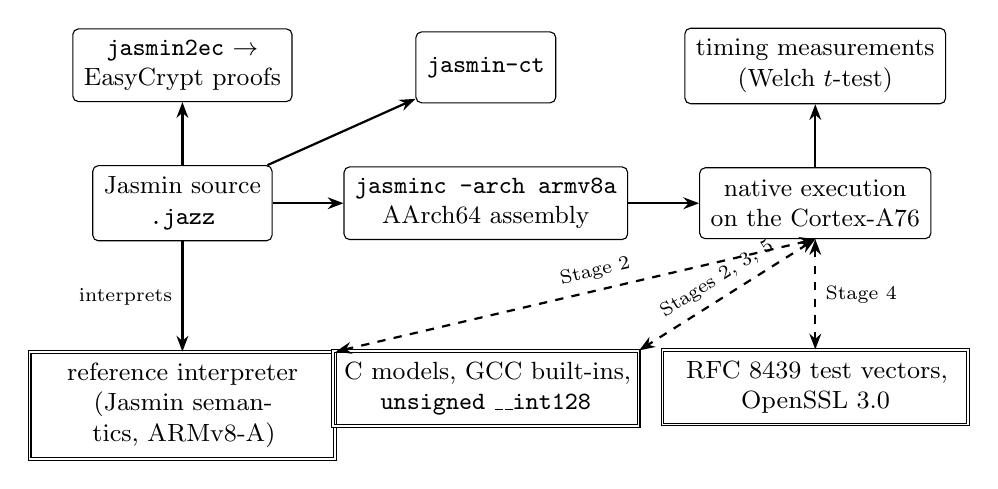
\begin{tikzpicture}[
  box/.style={draw, rounded corners=2pt, align=center,
              font=\small, minimum height=9mm, inner sep=4pt},
  orc/.style={draw, double, align=center,
              font=\small, minimum height=9mm, inner sep=4pt, text width=3.6cm},
  arr/.style={-{Stealth[length=2mm]}, thick},
  cmp/.style={{Stealth[length=2mm]}-{Stealth[length=2mm]}, thick, dashed},
  node distance=8mm and 9mm]
  \node[box] (src) {Jasmin source\\\texttt{.jazz}};
  \node[box, right=of src] (jc) {\texttt{jasminc -arch armv8a}\\AArch64 assembly};
  \node[box, right=of jc] (nat) {native execution\\on the Cortex-A76};
  \node[box, above=of src] (ec) {\texttt{jasmin2ec} $\to$\\EasyCrypt proofs};
  \node[box, above=of jc] (ct) {\texttt{jasmin-ct}};
  \node[box, above=of nat] (tm) {timing measurements\\(Welch $t$-test)};
  \node[orc, below=14mm of src] (interp) {reference interpreter\\(Jasmin semantics, ARMv8-A)};
  \node[orc, below=14mm of jc] (cm) {C models, GCC built-ins,\\\texttt{unsigned \_\_int128}};
  \node[orc, below=14mm of nat] (ossl) {RFC 8439 test vectors,\\OpenSSL 3.0};
  \draw[arr] (src) -- (jc);
  \draw[arr] (jc) -- (nat);
  \draw[arr] (src) -- (ec);
  \draw[arr] (src) -- (ct);
  \draw[arr] (nat) -- (tm);
  \draw[arr] (src) -- node[left, font=\scriptsize]{interprets} (interp);
  \draw[cmp] (nat.south) -- node[pos=0.45, above, font=\scriptsize, sloped]{Stage 2} (interp.north east);
  \draw[cmp] (nat.south) -- node[pos=0.5, above, font=\scriptsize, sloped]{Stages 2, 3, 5} (cm.north east);
  \draw[cmp] (nat.south) -- node[right, font=\scriptsize]{Stage 4} (ossl.north);
\end{tikzpicture}
\caption{Tools under test (single frame) and oracles (double frame). Solid
arrows show how the tools process the source program; dashed arrows denote
comparisons of results.}
\label{fig:oracles}
\end{figure}

\begin{itemize}[leftmargin=*,itemsep=1pt]
  \item The \textbf{reference interpreter} executes the \emph{source}
        program directly, with the ARMv8-A instruction semantics of the
        Jasmin library, that is, with the semantics to which the compiler
        correctness theorem refers. Agreement between the interpreter and
        the native execution therefore tests the entire chain: compiler,
        assembly printer, assembler, linker, ABI and processor.
  \item \textbf{Independent implementations} (C models, OpenSSL, RFC test
        vectors) additionally detect errors in the \emph{algorithms} of the
        test programs. The interpreter and the compiler process the same
        source program, so their agreement alone cannot detect such errors.
\end{itemize}

\subsection{Directory structure and usage}

\begin{lstlisting}[style=output]
armv8-tests/
|-- run-all.sh                # runs the 8 stages, prints [PASS]/[FAIL]/[INFO]
|-- results/run-all-output.txt
|-- lib/testlib.h             # PRNG (splitmix64), edge values, TL_CHECK
|-- tools/
|   |-- jasmin-interp/        # OCaml reference interpreter driver (dune)
|   |-- difftest.py           # interpreter-vs-native differential tester
|   `-- negtest.sh            # expected-failure runner
|-- 01-upstream/              # upstream tests (Jasmin v2026.09.0, MIT)
|-- 02-isa/                   # isa.jazz, test_models.c, test_ldst.c
|-- 03-abi/                   # trampoline.S, stackzero.jazz, test_abi.c
|-- 04-crypto/                # chacha20.jazz, poly1305.jazz + tests
|-- 05-ct/                    # ct.jazz, sct.jazz, test_ct.c
|-- 06-easycrypt/             # extracted/ (generated), proofs/
|-- 07-bench/                 # bench.c
|-- 08-negative/              # 17 programs the back end must reject
`-- report/                   # this document
\end{lstlisting}

The script \file{run-all.sh} runs all stages, or only the stages given as
arguments. It prints one line per check, marked \texttt{[PASS]},
\texttt{[FAIL]} or \texttt{[INFO]} (for measurements without a pass/fail
criterion), and a summary at the end:

\begin{lstlisting}[style=shell]
$ eval $(opam env --switch=jasmin-ec)
$ cd armv8-tests
$ ./run-all.sh                 # all stages (about 7 minutes)
$ ./run-all.sh 2 4             # only stages 2 and 4
\end{lstlisting}

Apart from the installation described in the installation guide, the tests
require only the Debian package \texttt{libssl-dev} (the development files
of OpenSSL). All random inputs originate from a pseudo-random generator with
a fixed seed, so that every run is reproducible.

%===========================================================================
\section{Stage 1: upstream tests on the ARMv8-A target}
%===========================================================================

\emph{Purpose: determine which of the test programs of the Jasmin
developers the ARMv8-A back end compiles, and whether the generated code is
valid ARMv8-A assembly.}

Three groups of tests were copied from the Jasmin v2026.09.0 sources: the 16
ARMv8-A-specific tests (\file{tests/success/armv8a}), the ARMv8-A
stack-zeroization test, and the 55 architecture-independent tests
(\file{tests/success/common}). The upstream test suite runs the \emph{common}
tests only for x86-64, ARM-M4 and RISC-V. Each program is compiled for
ARMv8-A and then assembled with the GNU assembler \texttt{as} (invoked
through \texttt{gcc -c}), which verifies that every emitted instruction can
be encoded as machine code:

\begin{lstlisting}[style=shell]
$ jasminc -arch armv8a -o build/up_add.s 01-upstream/armv8a/add.jazz
$ gcc -c -o build/up_add.o build/up_add.s
\end{lstlisting}

The stage also runs the upstream tests of the constant-time checker (in
the directories \file{CCT/success} and \file{CCT/fail}, which contain
programs that the checker must accept and programs that it must reject)
for the ARMv8-A architecture, and it translates the ARMv8-A programs to
EasyCrypt and type-checks the results. Table~\ref{tab:upstream} summarizes
the outcome.

\begin{table}[h]
\centering\small
\begin{tabularx}{\textwidth}{@{}Xrrl@{}}
\toprule
\textbf{Group} & \textbf{Programs} & \textbf{Passed} & \textbf{Remarks} \\
\midrule
\file{armv8a} & 16 & 16 & \\
\file{stack\_zeroization/armv8a} & 1 & 1 & \\
\file{common} (not run upstream for ARMv8-A) & 55 & 51 & 4 internal compiler errors \\
\file{CCT/success} with \texttt{jasmin-ct --arch=armv8a} & 15 & 15 & accepted \\
\file{CCT/fail} with \texttt{jasmin-ct --arch=armv8a} & 12 & 12 & rejected \\
extraction and EasyCrypt type check (\file{armv8a}, stack zeroization) & 17 & 17 & 6--10\,s each \\
\bottomrule
\end{tabularx}
\caption{Upstream tests on the ARMv8-A target.}
\label{tab:upstream}
\end{table}

\begin{finding}{1: internal compiler errors}
Four common tests (\file{bug\_499}, \file{renaming}, \file{swap},
\file{swap\_word}) cause the ARMv8-A back end to fail with an internal error:
\begin{lstlisting}[style=output]
"common/renaming.jazz", line 18 (2-21): internal compilation error in function mul:
  asmgen: assemble_sopn.pseudo_op: unexpected operator mulu_32
"common/swap.jazz", line 57 (2-21): internal compilation error in function wint:
  asmgen: assemble_sopn.pseudo_op: unexpected operator swap
\end{lstlisting}
Further tests (Stage~8) show that the 64-bit operation
\texttt{hi, lo = a * 64u b} (\texttt{mulu\_64}), which computes the full
128-bit product of two 64-bit numbers, fails in the same way. The x86-64
back end compiles all three operators. Because A64 provides the required
instructions (\texttt{UMULH}, \texttt{UMULL}), the errors reflect a missing
translation step (\emph{lowering}) in the back end rather than an
architectural limitation. They should be reported to the Jasmin developers
together with the reproducers in \file{08-negative/}.
\end{finding}

%===========================================================================
\section{Stage 2: differential testing}
%===========================================================================

\emph{Purpose: detect miscompilations by comparing the results of the
compiled code with the results that the language semantics prescribes.}

\subsection{A reference interpreter for ARMv8-A}

The Jasmin OCaml library contains an evaluator (module \texttt{Evaluator})
that executes a Jasmin program according to its formal semantics, but the
library provides no command-line program for it, and its test driver
supports only x86-64. A driver of 73 lines was therefore written. It loads a
program with the \emph{ARMv8-A} architecture definition, reads queries (a
function name and argument values) from standard input, and prints the
results:

\lstinputlisting[style=ocaml,firstline=17,lastline=73,caption={\file{tools/jasmin-interp/jasmin\_interp.ml} (main part)}]{../tools/jasmin-interp/jasmin_interp.ml}

\begin{lstlisting}[style=shell]
$ cd tools/jasmin-interp && dune build ./jasmin_interp.exe
$ printf 'add 1 2\ndiv 100 7\ndiv 5 0\n' | ./_build/default/jasmin_interp.exe add_div.jazz
add 0xdfadcefa
div 0x2
div ERROR arithmetic error
\end{lstlisting}

Division by zero is undefined in Jasmin, and the interpreter reports it as
an error. Such queries are excluded from the comparison, because the
semantics prescribes no result for them (the hardware returns 0). The
intrinsic \texttt{\#UDIV}, which models the hardware instruction, is defined
for a zero divisor, and its interpreted result agrees with the hardware.

\subsection{The differential tester}

The tester \file{tools/difftest.py} automates the comparison. It parses the
exported functions that take scalar arguments (\texttt{reg u8..u64}) and
return at most two scalar results. For these functions, it generates a C
program that calls the native code; a pair of results is returned as a
16-byte structure, that is, in the registers \texttt{x0} and \texttt{x1}.
The tester then generates queries, 30\,\% of which use edge values such as
$0, 1, 2^{63}$ and $2^{64}-1$ and the remainder uniformly distributed values,
submits them to both executions, and compares the results line by line:

\lstinputlisting[style=python,firstline=152,lastline=185,caption={\file{tools/difftest.py}: execution of both implementations and comparison}]{../tools/difftest.py}

\begin{lstlisting}[style=shell]
$ python3 tools/difftest.py 01-upstream/armv8a/div.jazz -n 2000 --show-undef
    undefined in Jasmin: div 0x8092b4d42b28fef0 0x0  -> interpreter: ERROR arithmetic error, native: 0x0
  [PASS] div.jazz:div  1970 agree, 30 undefined, 0 mismatch
$ python3 tools/difftest.py 01-upstream/armv8a/loop.jazz --bits loop=12   # bound the loop
\end{lstlisting}

The option \texttt{--bits} restricts an argument to a given number of bits;
it bounds, for example, the number of iterations of a loop whose trip count
is an argument.

\subsection{Instruction coverage beyond the upstream tests}

The upstream tests exercise only part of the instruction set. The file
\file{02-isa/isa.jazz} (17 functions, 264 lines) therefore covers further
instructions and constructs: 128-bit carry chains, subtraction with borrow,
a $64\times64 \to128$ product composed of 32-bit halves, \texttt{MADD} and
\texttt{MSUB} (multiply-add and multiply-subtract), constant and variable
rotations (64-bit and 32-bit), masked variable shifts, logical operations
with bitmask immediates, a SWAR population count (counting set bits with
word-parallel arithmetic), all ten comparison conditions, truncations and
sign and zero extensions, 32-bit wrap-around, loops with \texttt{UDIV}
(Euclid's algorithm), nested control flow (Collatz sequence), register
pressure with non-inlined calls, and stack and register arrays with dynamic
indices. The subtraction relies on the carry convention of A64, in which the
carry flag C after a subtraction is set when \emph{no} borrow occurs:

\lstinputlisting[style=jasmin,firstline=15,lastline=37,caption={\file{02-isa/isa.jazz}: borrow handling with the A64 carry flag}]{../02-isa/isa.jazz}

\begin{finding}{2: subtraction with borrow}
On ARMv8-A, the compiler rejects the generic Jasmin forms
\lstinline[style=jasmin,numbers=none,frame=none]|cf, a -= c; _, b -= d - cf;|
and \lstinline[style=jasmin,numbers=none,frame=none]|#sbb| with the message
\emph{``register allocation: variables \{cf; \_0\} remain unallocated''},
and it provides no \texttt{\#SBC} intrinsic. The workaround
(\texttt{SUBS}; \texttt{MVN}; \texttt{ADC}) relies on the A64 convention
``C = NOT borrow''. Section~\ref{sec:proofs} proves in EasyCrypt that the
flag returned by \texttt{\#SUBS} indicates $a \ge b$.
\end{finding}

\subsection{Independent C models}

Agreement between the interpreter and the native execution cannot reveal an
incorrect \emph{algorithm}, because both execute the same source program.
The program \file{02-isa/test\_models.c} therefore compares the arithmetic
functions with independent C implementations, which use the 128-bit type
\texttt{unsigned \_\_int128}, the GCC built-in function
\texttt{\_\_builtin\_popcountll}, and plain C, on $10^6$ inputs; the first
169 inputs enumerate all pairs of edge values. The program
\file{02-isa/test\_ldst.c} compares the two upstream functions that access
memory (\texttt{ldst}, \texttt{ldst32}) with C models. It compares the
complete 32-byte buffer, so that a store to a wrong address is also
detected.

\begin{table}[h]
\centering\small
\begin{tabular}{@{}lrrrr@{}}
\toprule
\textbf{Source} & \textbf{Functions} & \textbf{Inputs each} & \textbf{Undefined} & \textbf{Mismatches} \\
\midrule
upstream \file{armv8a} (scalar) & 18 & 2\,000 & 71 (division by 0) & 0 \\
\file{02-isa/isa.jazz} & 17 & 5\,000 & 0 & 0 \\
C models (\file{test\_models.c}) & 11 & $10^6$ & -- & 0 \\
memory functions (\file{test\_ldst.c}) & 2 & $10^6$ & -- & 0 \\
\bottomrule
\end{tabular}
\caption{Results of the differential tests. ``Undefined'' counts the queries
excluded because the language semantics prescribes no result.}
\end{table}

%===========================================================================
\section{Stage 3: AAPCS64 conformance}
%===========================================================================

\emph{Purpose: verify that Jasmin functions interoperate correctly with C
code, and that the erasure option removes secrets from the stack.}

A C caller relies on two rules of AAPCS64. First, a callee must preserve the
registers \texttt{x19}--\texttt{x29}, the lower halves of
\texttt{v8}--\texttt{v15} (\texttt{d8}--\texttt{d15}) and the stack pointer
\texttt{sp} (the \emph{callee-saved} registers): the caller may keep values
in them across the call. Second, a caller may pass 32-bit arguments in
64-bit registers whose upper halves contain arbitrary values; the callee
must ignore these halves. Neither rule can be tested from C, because the C
compiler controls the registers. Both rules were therefore tested with a
\emph{trampoline}, a small routine written in assembly that sets up the
registers, calls the Jasmin function, and inspects the registers afterwards:

\lstinputlisting[style=asm,firstline=21,lastline=40,caption={\file{03-abi/trampoline.S}: \texttt{abi\_call} (excerpt)}]{../03-abi/trampoline.S}

The routine \texttt{abi\_call} loads a distinct marker value into every
callee-saved register, calls the Jasmin function with \texttt{blr}, and
returns a bit mask of the registers whose contents changed. The routine
\texttt{abi\_call\_dirty32} sets the upper halves of \texttt{x0} and
\texttt{x1} to \texttt{0xdeadbeef} and \texttt{0xcafebabe} before it calls a
function with \texttt{u32} arguments. The routine \texttt{stack\_snapshot}
fills 1\,KiB below \texttt{sp} with the byte \texttt{0xAA}, calls the
function, and copies this area; the C test program then classifies every
64-bit word in the copy.

A function that stores secrets on the stack leaves them in memory after it
returns, where later code may read them. The Jasmin compiler can erase the
stack frame before returning (\emph{stack zeroization}), in a loop or with
unrolled stores. The program \file{03-abi/stackzero.jazz} distributes a
secret key over a 256-byte stack buffer, in three variants: without
zeroization, with \texttt{\#[stackzero=loop]}, and with
\texttt{\#[stackzero=unrolled]}.

\begin{table}[h]
\centering\small
\begin{tabularx}{\textwidth}{@{}XXr@{}}
\toprule
\textbf{Check} & \textbf{Functions} & \textbf{Result} \\
\midrule
x19--x29, d8--d15 and sp preserved & 8 (including 26 live values and calls) & 0 violations in 160\,000 calls \\
undefined upper halves of 32-bit arguments & 6 & 0 differences in 1\,200\,000 calls \\
\bottomrule
\end{tabularx}

\vspace{6pt}
\begin{tabular}{@{}lrrrr@{}}
\toprule
\textbf{Stack after return} & \textbf{Secret words} & \textbf{Return address} & \textbf{Zero words} & \textbf{Other} \\
\midrule
without zeroization & 31 & 1 & 1 & 0 \\
\texttt{stackzero=loop} & \textbf{0} & 1 & 32 & 0 \\
\texttt{stackzero=unrolled} & \textbf{0} & 1 & 32 & 0 \\
\bottomrule
\end{tabular}
\caption{Results of the ABI and stack-zeroization tests.}
\end{table}

The single remaining word is the link register (the return address), which
the function saves with \texttt{str x30, [sp, \#-16]!}; it is a public code
address outside the erased frame. Without zeroization, 31 of the 32
secret-derived words remain readable after the call; the 32nd word equals
$k \oplus k = 0$.

\begin{note}
The compiler rejects \texttt{\#[stackzero=loopSCT]}, the variant that is
hardened against speculative execution, on ARMv8-A: \emph{``Strategy "loop
with SCT" is not supported in ARMv8-A''}.
\end{note}

%===========================================================================
\section{Stage 4: cryptographic kernels}
%===========================================================================

\emph{Purpose: verify that the back end compiles complete cryptographic
algorithms correctly, by comparison with standardized test vectors and with
an established library.}

ChaCha20 is a stream cipher, and Poly1305 is a message authentication code;
RFC~8439 standardizes both, and they are widely used together (for example
in TLS). Both were implemented in Jasmin for this stage.

\subsection{ChaCha20}

The ChaCha20 block function transforms a state of 16 words of 32 bits in 20
rounds. The Jasmin implementation holds the state in 32-bit (W) registers.
The 32-bit rotations compile to the instruction \texttt{ror}, and the
pointer arguments are stored on the stack during the 20 rounds:

\lstinputlisting[style=jasmin,firstline=1,lastline=50,caption={\file{04-crypto/chacha20.jazz} (rounds; the feed-forward follows)}]{../04-crypto/chacha20.jazz}

\subsection{Poly1305 without a wide multiplier}

Poly1305 evaluates a polynomial modulo the prime $2^{130}-5$. The usual
64-bit implementation represents 130-bit numbers in three 64-bit limbs and
requires $64\times64\to128$ products. Because \texttt{mulu} causes an
internal compiler error (Finding~1), the implementation instead represents
the accumulator in radix $2^{26}$, that is, in five limbs of 26 bits. Every
partial product then fits into a 64-bit register, and \texttt{MADD}
(multiply-add) accumulates it:

\lstinputlisting[style=jasmin,firstline=24,lastline=50,caption={\file{04-crypto/poly1305.jazz}: processing of one block}]{../04-crypto/poly1305.jazz}

The final reduction (subtraction of $2^{130}-5$ if $h \ge 2^{130}-5$) is a
branch-free selection with a mask. Loops with a public length assemble the
last partial block of the message byte by byte.

\subsection{Results}

\begin{table}[h]
\centering\small
\begin{tabularx}{\textwidth}{@{}lXr@{}}
\toprule
\textbf{Kernel} & \textbf{Oracle} & \textbf{Result} \\
\midrule
ChaCha20 block & RFC 8439 \S2.3.2 test vector & \yes \\
ChaCha20 block & OpenSSL \texttt{EVP\_chacha20}: random key and nonce; counters $0$, $2^{32}-1$ and random & 200\,000 / 200\,000 \\
Poly1305 & RFC 8439 \S2.5.2 test vector & \yes \\
Poly1305 & OpenSSL \texttt{EVP\_MAC("POLY1305")}: lengths 0..300; random, 0x00 and 0xff data & 62\,608 / 62\,608 \\
\bottomrule
\end{tabularx}
\caption{Cryptographic kernels compared with RFC 8439 and OpenSSL 3.0.20.}
\end{table}

Messages and keys that consist of \texttt{0xff} bytes bring the accumulator
close to the modulus and thereby exercise the final conditional
subtraction, which random data rarely reach.

%===========================================================================
\section{Stage 5: constant time}
%===========================================================================

\emph{Purpose: verify that the constant-time checker classifies
constant-time and leaky code correctly on ARMv8-A, and that the processor
behaves accordingly.}

\subsection{Static verification with \texttt{jasmin-ct}}

\texttt{jasmin-ct} offers three modes. The default mode (CT) checks that
secrets influence neither branches nor memory addresses. The mode
\texttt{--doit} additionally requires that secrets be processed only by
instructions whose timing the architecture guarantees to be independent of
their operands (data-operand-independent timing, DOIT). The mode \texttt{--sct} checks speculative constant time; programs
achieve this property with speculative load hardening.

The file \file{05-ct/ct.jazz} pairs three constant-time kernels with leaky
counterparts: buffer comparison (without and with early exit), conditional
swap (masking and branching), and table lookup (scan of the whole table with
\texttt{CSEL} and direct indexing with the secret index). A function that
divides by a secret completes the set. Annotations declare the security
types. Pointers are public, and the memory to which they point is secret by
default:

\lstinputlisting[style=jasmin,firstline=75,lastline=103,caption={\file{05-ct/ct.jazz}: table lookup by scan and by direct indexing}]{../05-ct/ct.jazz}

\begin{table}[h]
\centering\small
\begin{tabular}{@{}lccc@{}}
\toprule
\textbf{Function} & \texttt{jasmin-ct} & \texttt{--doit} & \texttt{--sct} \\
\midrule
\texttt{ct\_memeq}, \texttt{ct\_cswap4}, \texttt{ct\_lookup16} & \yes & \yes & \no{} (no SLH) \\
\texttt{chacha20\_block}, \texttt{poly1305} & \yes & \yes & \no{} (no SLH) \\
\texttt{leaky\_memeq} (secret branch) & \no & & \\
\texttt{leaky\_cswap4} (secret branch) & \no & & \\
\texttt{leaky\_lookup16} (secret address) & \no & & \\
\texttt{leaky\_div} (secret divisor) & \no & & \\
\texttt{sct\_memeq}, \texttt{sct\_lookup16} (\file{sct.jazz}, SLH) & & & \yes \\
\bottomrule
\end{tabular}
\caption{Verdicts of \texttt{jasmin-ct --arch=armv8a} (\yes{} accepted, \no{} rejected); all verdicts are as expected.}
\end{table}

\begin{finding}{3: no speculative load hardening on ARMv8-A}
The file \file{05-ct/sct.jazz} hardens \texttt{memeq} and \texttt{lookup16}
with SLH: \texttt{\#init\_msf} and \texttt{\#update\_msf} maintain a
\emph{misspeculation flag}, which records whether the processor is
executing a mispredicted branch, and \texttt{\#protect} masks values with
this flag so that misspeculated loads cannot leak secrets.
\texttt{jasmin-ct --sct --arch=armv8a} accepts the file, and
\texttt{jasminc -arch x86-64} compiles it, but the ARMv8-A back end rejects
it:
\begin{lstlisting}[style=output]
$ jasminc -arch armv8a 05-ct/sct.jazz
speculative execution lowering: The architecture does not provides protection
for selective speculative load hardening
\end{lstlisting}
All 24 upstream SLH tests (\file{tests/success/slh}) fail in the same way on
ARMv8-A. Protection against Spectre v1 is therefore not yet available for
this target, although AArch64 provides the necessary means (\texttt{CSDB}
and conditional selection). In addition, the SLH lowering recognizes only
loop conditions that are bound to a Boolean variable, as in
\lstinline[style=jasmin,numbers=none,frame=none]|while {c = i < n;} (c)|.
\end{finding}

\subsection{Timing measurements}

The static checks concern the program; the actual timing behavior depends
on the processor. The timing of the hardware was therefore measured with the
method of the tool \emph{dudect}: two classes of inputs (for example, two
equal buffers and two buffers that differ in the first byte) are
interleaved at random, each execution is timed, and the two distributions of
execution times are compared with Welch's $t$-test. The timer is the ARMv8
virtual counter \texttt{CNTVCT\_EL0} (54\,MHz), read after the barrier
instruction \texttt{isb}. Following the threshold customary in leakage
assessment (TVLA), a statistic $|t| > 4.5$ is taken as evidence of a timing
difference, that is, of a leak.

\lstinputlisting[style=c,firstline=19,lastline=41,caption={\file{05-ct/test\_ct.c}: timer and Welch statistic}]{../05-ct/test_ct.c}

\begin{table}[h]
\centering\small
\begin{tabular}{@{}lllrrr@{}}
\toprule
\textbf{Function} & \textbf{Class 0} & \textbf{Class 1} & \textbf{Ticks (class 0)} & \textbf{Ticks (class 1)} & $|t|$ \\
\midrule
\texttt{ct\_memeq} (4\,KiB) & equal & differ at byte 0 & 919.3 & 907.2 & 0.65 \\
\texttt{leaky\_memeq} & equal & differ at byte 0 & 1504.8 & 2.3 & \textbf{408.77} \\
\texttt{ct\_cswap4} ($\times$256) & $c=0$ & $c=1$ & 72.2 & 72.1 & 0.45 \\
\texttt{leaky\_cswap4} ($\times$256) & $c=0$ & $c=1$ & 24.9 & 56.2 & \textbf{65.25} \\
\bottomrule
\end{tabular}
\caption{Timing tests (20\,000 samples per class; ticks of the 54\,MHz
counter). The verdicts agree with those of \texttt{jasmin-ct}.}
\end{table}

%===========================================================================
\section{Stage 6: EasyCrypt}
\label{sec:proofs}
%===========================================================================

\emph{Purpose: verify that the translation of ARMv8-A programs to EasyCrypt
works, and prove constant time and functional correctness formally.}

\subsection{Extraction}

Each of the five test programs is translated twice for ARMv8-A: once as a
plain EasyCrypt module, and once with the option \texttt{-m CT}, which
produces a \emph{leakage model}: every procedure additionally returns its
leakage (branch conditions, memory addresses, loop bounds) as part of its
result. All ten files type-check against the eclib model
\file{JModel\_armv8a.ec}:

\begin{lstlisting}[style=shell]
$ jasmin2ec --arch=armv8a       -o 06-easycrypt/extracted/Ct.ec    05-ct/ct.jazz
$ jasmin2ec --arch=armv8a -m CT -o 06-easycrypt/extracted/Ct_CT.ec 05-ct/ct.jazz
$ cd 06-easycrypt/extracted && easycrypt compile -no-eco Ct_CT.ec
\end{lstlisting}

\begin{table}[h]
\centering\small
\begin{tabular}{@{}lrr@{}}
\toprule
\textbf{Program} & \textbf{Lines (plain model)} & \textbf{Lines (leakage model)} \\
\midrule
\file{isa.jazz} & 390 & 494 \\
\file{stackzero.jazz} & 48 & 75 \\
\file{chacha20.jazz} & 134 & 272 \\
\file{poly1305.jazz} & 293 & 583 \\
\file{ct.jazz} & 115 & 221 \\
\bottomrule
\end{tabular}
\caption{Extracted EasyCrypt models (each model type-checks in about 10\,s).}
\end{table}

\subsection{Constant-time proofs}

Constant time is a \emph{2-safety} property: it relates two executions
rather than one. Two executions that agree on the public inputs must
produce the same leakage, \emph{regardless of the secrets}. In pRHL, which
relates two programs, this property is an \texttt{equiv} judgment whose
precondition equates only the public arguments and whose postcondition
equates the leakage. The precondition does not equate the memory
(\texttt{Glob.mem}), so keys and messages may differ between the two
executions:

\lstinputlisting[style=easycrypt,caption={\file{06-easycrypt/proofs/ct\_proofs.ec}}]{../06-easycrypt/proofs/ct_proofs.ec}

All five proofs are checked in 11\,s. For \texttt{ct\_lookup16}, the proof
confirms that the comparison \texttt{i = idx} is an operand of a
\texttt{CSEL}, not a branch condition, and therefore does not appear in the
leakage. For the three leaky functions, the same proof scripts must fail,
and they do (\file{proofs/fail\_leaky\_*.ec}):

\begin{lstlisting}[style=shell]
$ easycrypt compile -no-eco -I extracted proofs/fail_leaky_memeq.ec
[critical] [proofs/fail_leaky_memeq.ec: line 11 (0-58)] [by]: cannot close goals
\end{lstlisting}

\subsection{Functional correctness of the carry handling}

The ARMv8-A model defines \texttt{SUBS} (subtraction that sets the flags)
as \texttt{ADCS x (invw y) true}, that is, as an addition of the bitwise
complement with an incoming carry, in accordance with the A64 carry
convention. The proofs establish that the 128-bit addition of
\file{isa.jazz} is exact modulo $2^{128}$ and that the flag returned by
\texttt{\#SUBS} is set exactly when no borrow occurs. These results justify
the workaround of Finding~2:

\lstinputlisting[style=easycrypt,firstline=38,lastline=74,caption={\file{06-easycrypt/proofs/isa\_correct.ec} (main lemmas)}]{../06-easycrypt/proofs/isa_correct.ec}

The two auxiliary integer lemmas (\texttt{mod\_split}, \texttt{carry\_div})
are proved in the same file, which is checked in 14\,s.

\begin{note}
When a tactic fails, \texttt{easycrypt compile} prints only the error. To
inspect proof goals without an editor, pass a prefix of the file to
\cmd{easycrypt cli -emacs -I extracted}. The proofs of this stage were
developed in this way on the Raspberry Pi.
\end{note}

%===========================================================================
\section{Stage 7: performance}
%===========================================================================

\emph{Purpose: compare the speed of the code generated by the ARMv8-A back
end with that of C and of optimized libraries.}

The program \file{07-bench/bench.c} measures throughput as the median of
11 runs and reports it in nanoseconds per byte and in processor cycles per
byte at 2.4\,GHz (lower values are better). For comparison, it measures
portable C implementations of the \emph{same algorithms} (scalar ChaCha20,
Poly1305 in radix $2^{26}$) and OpenSSL, which uses hand-written NEON
(vector) and scalar assembly:

\begin{table}[h]
\centering\small
\begin{tabular}{@{}llrr@{}}
\toprule
\textbf{Kernel} & \textbf{Implementation} & \textbf{ns/byte} & \textbf{Cycles/byte} \\
\midrule
ChaCha20, 1 block & Jasmin (scalar) & 2.86 & 6.86 \\
                  & C, \texttt{gcc -O2} (scalar) & 2.50 & 6.01 \\
                  & OpenSSL, 64-byte calls & 2.64 & 6.33 \\
ChaCha20, 4\,KiB  & OpenSSL (NEON, several blocks) & 1.00 & 2.40 \\
\midrule
Poly1305, 4\,KiB  & Jasmin (radix $2^{26}$, 64-bit \texttt{MADD}) & 2.27 & 5.45 \\
                  & C, \texttt{gcc -O2} (radix $2^{26}$, \texttt{UMADDL}) & 0.91 & 2.17 \\
                  & OpenSSL & 0.50 & 1.21 \\
\bottomrule
\end{tabular}
\caption{Throughput on the Cortex-A76. The Jasmin results do not depend on
the C compiler flags; with \texttt{-O3}, the C results differ by less than
3\,\%.}
\end{table}

The scalar ChaCha20 implementation in Jasmin is within 15\,\% of the code
generated by GCC. A faster implementation would require NEON, which this
release of the back end does not support (it has no vector registers).

\begin{finding}{4: UMULL and UMADDL modeled but not available}
The inner loop of Poly1305 comprises about 90 instructions per 16 bytes and
causes no stack traffic. The difference from C originates in the
multiplications: GCC emits 25 \texttt{umaddl} and \texttt{umull}
instructions, which multiply two 32-bit values into a 64-bit result, whereas Jasmin can
emit only the 64-bit \texttt{madd}, which has a longer latency on the
Cortex-A76. The eclib model already defines these instructions
(\texttt{op UMULL} and \texttt{op UMADDL} in \file{JModel\_armv8a.ec}), but
the compiler rejects them with the message \emph{``unknown primitive:
"UMULL"''}. Making them available, together with \texttt{UMULH} for
\texttt{mulu}, would remove most of the difference.
\end{finding}

%===========================================================================
\section{Stage 8: limitations of the back end}
%===========================================================================

\emph{Purpose: record every limitation found during the campaign in a form
that detects its removal in a future release.}

Each limitation has a minimal reproducer in \file{08-negative/}: a small
program that the back end must reject. Each reproducer states the expected
error message in a comment line that begins with \texttt{// EXPECT:}, and
\file{tools/negtest.sh} verifies that \texttt{jasminc -arch armv8a} rejects
the program with a matching message. If a future release removes a
limitation, the corresponding program compiles, and the test fails; the
change is therefore noticed. For comparison, the last column of the table
indicates whether the x86-64 back end accepts the same program.

\begin{longtable}{@{}p{2.9cm}p{8.1cm}p{2.4cm}c@{}}
\toprule
\textbf{Test} & \textbf{Limitation (ARMv8-A)} & \textbf{Workaround} & \textbf{x86} \\
\midrule
\endhead
\texttt{mulu64} & \ice: $64\times64\to128$ \texttt{hi, lo = a * 64u b} & radix $2^{26}$ or 32-bit halves & \yes \\
\texttt{mulu32} & \ice: $32\times32\to64$ into two registers & \texttt{(64u)} casts & \yes \\
\texttt{swap32} & \ice: \texttt{\#swap} on \texttt{u32} (the 64-bit form works) & 64-bit swap & \yes \\
\texttt{sbb} & generic borrow: the flag cannot be allocated & \texttt{SUBS}+\texttt{MVN}+\texttt{ADC} & \yes \\
\texttt{slh} & no SLH (\texttt{init\_msf}, \texttt{protect}) & none & \yes \\
\texttt{stackzero\_\-loopsct} & \texttt{stackzero=loopSCT} not supported & \texttt{loop}, \texttt{unrolled} & \yes \\
\texttt{umull} & \texttt{UMULL} and \texttt{UMADDL} are not intrinsics (but are defined in eclib) & 64-bit \texttt{MUL} & -- \\
\texttt{vector} & no vector (NEON) registers & scalar code & \yes \\
\texttt{u8\_arith} & no 8-bit or 16-bit registers & 32-bit or 64-bit operations & \yes \\
\texttt{args9} & at most 8 arguments (no arguments on the stack) & pass a pointer & \no \\
\texttt{adc\_imm} & \texttt{ADC} has no immediate form & register & \yes \\
\texttt{mul\_imm} & \texttt{MUL} has no immediate form & register & \yes \\
\texttt{add32\_imm} & 32-bit \texttt{ADD}: only 12-bit immediates (handled automatically for 64-bit) & register & \no \\
\texttt{logic\_imm} & logical operations: only bitmask immediates & register & \yes \\
\texttt{csel\_imm} & conditional move of an immediate & register & \no \\
\texttt{shift\_unmasked} & a variable shift must have the form \texttt{x << (n \& 63)} & mask & \no \\
\texttt{rotl\_var} & no rotation to the left by a register & \texttt{>>r} by $-n$ & \no \\
\bottomrule
\caption{Expected compilation failures (all 17 programs are rejected with the
expected message). \ice{} denotes an internal compiler error. In the x86
column, \yes{} means that the x86-64 back end accepts the program and \no{}
that it rejects it as well.}
\end{longtable}

The upper part of the table lists features that the back end lacks. The
lower part follows from the A64 instruction set or from Jasmin's deliberate
rule that each source instruction corresponds to exactly one machine
instruction. These restrictions are intended, but users familiar with
x86-64 may not expect them: on x86-64, for example, \texttt{a * 3} and
\texttt{\_, c += 0 + cf} are valid.

%===========================================================================
\section{Conclusion and recommendations}
%===========================================================================

On the Raspberry Pi~5, the ARMv8-A back end of Jasmin 2026.09.0 generated
correct code for every test program that it accepted. This result covers the 72
upstream programs, the 17 instruction-coverage functions, the ABI tests and
two complete RFC~8439 primitives. In more than $10^7$ executions, no result
disagreed with the language semantics or with OpenSSL. The generated code
conforms to the calling convention, stack zeroization is effective, and the
constant-time guarantees hold statically, empirically and in EasyCrypt
proofs on the extracted leakage model.

The back end is nevertheless at an early stage of development. The following
actions are recommended:
\begin{enumerate}[leftmargin=*,itemsep=1pt]
  \item \textbf{Report} the three internal compiler errors
        (\file{08-negative/mulu64.jazz}, \file{mulu32.jazz},
        \file{swap32.jazz}) and the register-allocation failure for borrows
        (\file{sbb.jazz}) to the Jasmin developers.
  \item Do \textbf{not} yet rely on protection against Spectre v1 on
        ARMv8-A: the checker accepts SLH programs that the compiler cannot
        compile.
  \item Use the workarounds of Stage~8 for wide multiplications and
        borrows. This test suite covers their correctness, and an EasyCrypt
        proof additionally covers the borrow.
  \item Rerun \file{run-all.sh} after each upgrade of Jasmin. The
        expected-failure tests detect every limitation that a new release
        removes.
\end{enumerate}

The third document of this repository (\file{../NTRU+}) uses a development
version of the back end with NEON support, which removes the limitation
\texttt{vector} of Stage~8, to implement the vector kernels of a
post-quantum key encapsulation mechanism.

%===========================================================================
\appendix
\section{Glossary}
\label{app:glossary}
%===========================================================================

\begin{small}
\begin{description}[leftmargin=0pt,itemsep=2pt]
  \item[A64] The instruction set of AArch64.
  \item[Borrow] The bit that a subtraction takes from the next higher limb
        when its result would be negative.
  \item[Callee-saved register] A register whose value a called function must
        restore before it returns.
  \item[dudect] A method and tool for detecting timing leaks by statistical
        comparison of the execution times of two input classes.
  \item[eclib] The EasyCrypt library of Jasmin, which models machine words
        and instructions.
  \item[Extraction] The translation of a Jasmin program into an EasyCrypt
        module by \texttt{jasmin2ec}.
  \item[Immediate] A constant operand encoded directly in an instruction.
  \item[Intrinsic] A Jasmin operator that corresponds to one specific machine
        instruction, written with the prefix \texttt{\#}.
  \item[Lowering] A compiler step that replaces a high-level operation by
        machine instructions.
  \item[Radix $2^{26}$] A representation of a large integer by limbs of
        26 bits each.
  \item[Reproducer] A minimal program that triggers a specific behavior of
        the compiler.
  \item[Stack zeroization] The erasure of a function's stack frame before the
        function returns.
  \item[Trampoline] A small assembly routine that sets up the processor
        state, calls another function, and inspects the state afterwards.
  \item[2-safety] A property that relates two executions of the same
        program, such as constant time.
\end{description}
\end{small}

%===========================================================================
\section{Complete output of \texttt{run-all.sh}}
\label{app:output}
%===========================================================================

\lstinputlisting[style=output]{../results/run-all-output.txt}

\end{document}
